\documentclass[./../main.tex]{subfiles}
\graphicspath{{img/}}
\begin{document}
	\begin{exercise}
		Determina el momento de inercia del núcleo de \ch{^{170}Hf} de acuerdo a la \cref{fig:hafmio-rot-spectrum}, un valor por cada energía y \(J^{\pi}\) o si deseas puedes hacer una gráfica \(J^{\pi}\) vs. \(E\).

		\begin{figure}[htb]
			\centering
			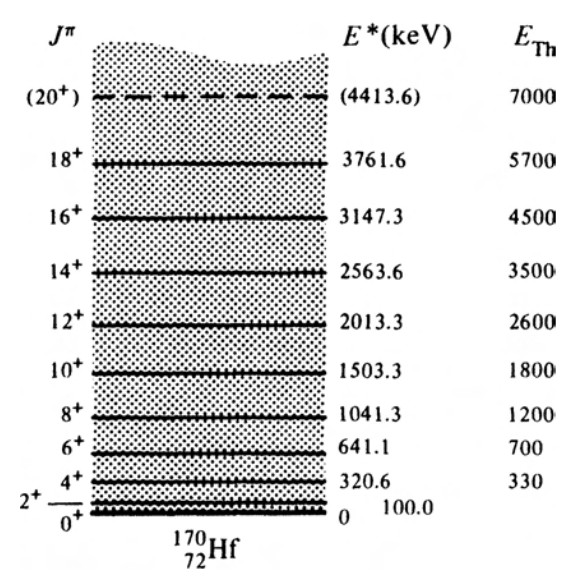
\includegraphics[scale=0.4]{rot_spectrum}
			\caption{Espectro rotacional del núcleo deformado \ch{^{170}Hf}.}			
			\label{fig:hafmio-rot-spectrum}
		\end{figure}

		\begin{solution}
			Sabemos que los eigenvalores de energía rotacionales están dados por

			\begin{equation*}
				E_{J} = \dfrac{\hbar^{2}}{2\mathcal{I}}J(J + 1),\quad J = 0, 2, 4, \ldots
			\end{equation*}

			Pero queremos conocer el momento de inercia \(\mathcal{I}\), por lo que despejando obtenemos

			\begin{equation*}
				\mathcal{I} = \dfrac{\hbar^{2}}{2E_{J}}J(J + 1), \quad J = 0, 2, 4, \ldots
			\end{equation*}

			donde \(\hbar = \qty{6.582119e-19}{\keV\s}\).

			\pagebreak
			De esta manera, podemos calcular el momento de inercia para cada valor de \(J\) y \(E_{J}\) de la \cref{fig:hafmio-rot-spectrum}.

			\begin{table}[htb]
                \centering
                \begin{tblr}{
                    colspec = {ccc},
                    hlines,
                    vlines,
					cell{1}{-} = {r=2}{c, m},
                }
                    \(J^{\pi}\)    & {Energía\\ (\unit{\keV})}   &  {\(\mathcal{I}\)\\ (\unit{\keV\s\squared})} \\
								   & 							 &												\\
                    \(2^{+}\)      &   \num{100}    			 &  \num{1.29973e-38}			   				\\
                    \(4^{+}\)      &   \num{320.6}    			 &  \num{1.35135e-38}							\\
                    \(6^{+}\)      &   \num{641.1}    			 &  \num{1.41914e-38}							\\
                    \(8^{+}\)      &   \num{1041.3}    			 &  \num{1.49781e-38}							\\
                    \(10^{+}\)     &   \num{1503.3}    			 &  \num{1.58507e-38}                           \\
                    \(12^{+}\)     &   \num{2013.3}    			 &  \num{1.67849e-38}							\\
                    \(14^{+}\)     &   \num{2563.6}    			 &  \num{1.77448e-38}							\\
                    \(16^{+}\)     &   \num{3147.3}    			 &  \num{1.87211e-38}							\\
                    \(18^{+}\)     &   \num{3761.6}    			 &  \num{1.96949e-38}							\\
                    \(20^{+}\)     &   \num{4413.6}    			 &  \num{2.06138e-38}							\\
                \end{tblr}
                \caption{Momentos totales de inercia con su respectiva energía y momento de inercia \(I\) para el \ch{^{170}Hf}.}
				\label{tblr:momentOfInertia}
            \end{table}

			Graficando los valores de \(J^{\pi}\) vs. \(E_{J}\) y de \(\mathcal{I}\) vs. \(E_{J}\) a partir de los datos de la \cref{tblr:momentOfInertia}, obtenemos la \cref{fig:Jpi-IVSEnergy}.

			\begin{figure}[!htb]
				\centering
				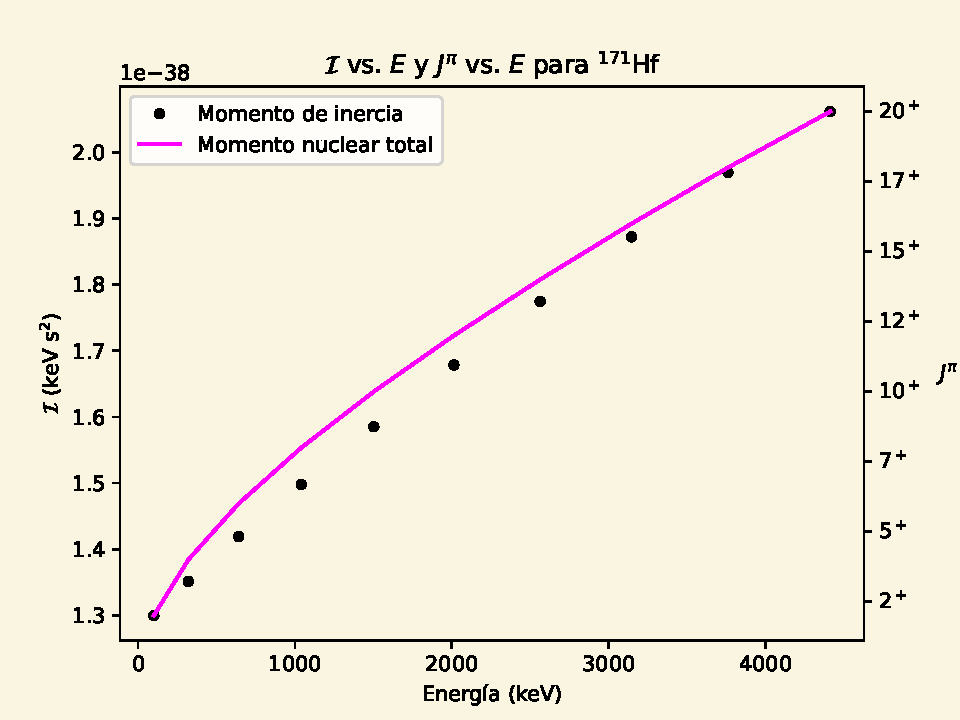
\includegraphics[scale=0.85]{moment_of_inertia.pdf}
				\caption{Gráfica de \(J^{\pi}\) vs. \(E_{J}\) y de \(\mathcal{I}\) vs. \(E_{J}\) para el \ch{^{170}Hf}}.
				\label{fig:Jpi-IVSEnergy}
			\end{figure}

			Como podemos observar, tanto el momento nuclear total \(J^{\pi}\) como el momento de inercia \(\mathcal{I}\) aumentan conforme aumenta la energía \(E_{J}\).
		\end{solution}
	\end{exercise}
\end{document}
